\section{\huge{Bonusopgaver}}

\subsection{Den hyggelige opgave}

Forbind prikkerne.

\begin{center}
\includegraphics[width=.99\textwidth]{forbind-prikkerne.pdf}
\end{center}


\newpage
\subsection{Rus opgaven}
Udtryk funktionen \texttt{fold} udelukkende ved hjælp af
\texttt{foldBack} og uden eksplicit rekursion.
Husk at \texttt{foldBack} og \texttt{fold} i F\# begge har typen
\begin{verbatim}
('State -> 'T -> 'State) -> 'State -> 'T list -> 'State
\end{verbatim}

\subsection{2. års rus opgaven}
Som storkunde hos internetudbyderen IP Factory har du har fået tildelt IP-adresseblokken 200.23.18.0/23.
Hvor mange forskellige IP-adresser råder du over? Angiv også den højeste og den laveste IP-adresse i dit råderum.

\subsection{3. års rus opgaven}
Konstruer en SLR-parsertabel for følgende grammatik:

\[
S \rightarrow \texttt{torben}\ S'\ \texttt{og}\ \texttt{fritz}
\]
\[
S \rightarrow \texttt{torben}\ F\ \texttt{og}\ \texttt{torben}
\]
\[
F \rightarrow S''\ \texttt{fritz}\ S''\ \texttt{fritz}\ S\ |\ \texttt{torben}\ \texttt{, }\ F
\]
\[
S' \rightarrow \epsilon\ |\ \texttt{, }\ S
\]
\[
S'' \rightarrow \texttt{, }\ |\ \texttt{, }\ S\ \texttt{, }
\]

\newpage

\subsection{De små opgaver}
\vspace{-0.1cm}

\subsubsection{Underopgave 0}
\vspace{-0.2cm}

Donald kan godt lide primtal, men kender kun primtallene op til 2. Hjælp ham
ved at lave en F\# (eller SML) funktion, der finder alle primtal under 100.

\subsubsection{Underopgave 1}

Donald elsker IEEE standarder og har for nyligt fundet IEEE 754 til
repræsentation af tal. Hjælp ham med at omskrive tallet $173.8$ til dets
32-bit IEEE 754 repræsentation. Blev der mistet præcision?


\subsubsection{Underopgave 2}
\vspace{-0.2cm}

Implementér en x64-simulator i C.

Husk at indentere med mellemrum og ikke lave for lange linjer.

\subsubsection{Underopgave 3}
\vspace{-0.2cm}

Håndkør følgende Whitespace-program og rapportér dets output:
\begin{verbatim}





\end{verbatim}

\newpage
\subsection{C opgaven}
For at undgå flaskehalse har Kantinebestyrelsen anskaffet sig en ny colaautomat
med et flerbrugersystem, så nu kan $n > 1$ brugere købe cola fra den samme
automat samtidigt.  Automaten blev leveret med følgende enterprise-kode:
\begin{verbatim}
int antal_colaer = 1000;

void køb_en_cola() {
  afspil_fanfare();
  if (antal_colaer > 0) {
    træk_kroner(15);
    antal_colaer--;
    giv_cola();
  }
}
\end{verbatim}
Antag at koden køres samtidigt af flere brugere.  Lokalisér kapløbsstriden og
reparér den med en lås.

\textbf{Avanceret:} Hvordan kunne du løse dette problem ved brug af DCR grafer?

\newpage

% Den skægge opgave lavet af Niels
\subsection{Den skægge opgave}

Preben har fået et lækkert $1 \times 1$ stykke chokolade i Julagave. Preben er
dog en flink fyr, så han vil gerne dele sin chokolade med sine venner.
Da Preben er en populær fyr, har han igennem sin tid på DIKU, fået uendelige
venner (Ja, så mange starter der hvert år\ldots).\\
\noindent Han vil gerne beholde halvdelen ($\frac{1}{1} \times \frac{1}{2}$) til
sig selv.
Derefter vil han gerne give sin bedste ven et stykke der er $\frac{1}{2} \times
\frac{1}{3}$. Han har nøge rangeret, hvor gode venner han er med hver person.
Han vil derfor give $\frac{1}{k} \times \frac{1}{k + 1}$ stykke chokolade, til
sin $k$ bedste ven.\\


\textbf{Din opgave:}
\begin{quote}
\noindent Kan alle hans venner få et sykke af chokoladen, eller når Preben at
løbe tør, før alle har fået?
\begin{figure}[h]
    \centering
    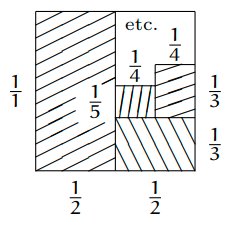
\includegraphics[width=0.5\textwidth]{preben.png}
\end{figure}
\end{quote}

\textbf{\emph{NB:\@ Der udloddes en flaske snaps til den første som kommer op i
baren med en korrekt besvarelse af denne opgave!}}
